% RIT ALGO2e strategy report: body only. Use % RIT ALGO2e strategy report: body only. Use % RIT ALGO2e strategy report: body only. Use % RIT ALGO2e strategy report: body only. Use \input{strategy_report_body} inside your document.
% Needs in the preamble: amsmath, booktabs, tabularx, graphicx, float, caption, subcaption, xcolor, listings, enumitem
\providecommand{\code}[1]{\texttt{#1}}
\section*{RIT ALGO2e: Strategy Report}
\addcontentsline{toc}{section}{RIT ALGO2e: Strategy Report}
Main strategy: \code{algo2e\_fin.py} (trading code in Appendix~\ref{app:code}).


%==========================================================================================
\subsection*{(a) What was your strategy going in?}

\textbf{The problem.} ALGO2e is a liquidity-provision case: three stocks (CNR $\approx$\$160, RY $\approx$\$100, AC $\approx$\$25), a 25{,}000-share gross and net
limit with fines for breaches, and a fee schedule that pays a rebate for resting orders on two of the three stocks. Market making is the natural way to earn money
here: quote a bid and an ask, collect the spread and the rebate, and keep inventory near zero. It is also the natural way to lose money, because in a trending market
a market maker keeps buying a falling price (or selling a rising one) and ends up holding a large position against the move. We did not know in advance which kind
of market the case would produce. Our working guess was that prices would mostly mean-revert around an anchor, with the possibility of trends or shocks injected during
the case. The strategy therefore had to make money in a calm market, survive a trending one, and switch between the two without anyone touching it.

\textbf{The design: a regime-switching system with three parts.}
\begin{enumerate}
  \item \textbf{Market maker (base income in calm markets).} Passive quotes on every stock, sized according to how volatile the stock currently is, with an
        inventory brake that makes it progressively harder to add to a position and easier to reduce it.
  \item \textbf{Trend engine (insurance against our guess being wrong).} When a stock starts moving steadily in one direction, quoting on that stock stops and
        the engine takes a large position \emph{with} the move, held with a trailing stop that is scaled to the stock's volatility.
  \item \textbf{Risk layer (overrides both).} Only limit orders are used, every order is checked against worst-case exposure before it is sent, and an account-level
        circuit breaker and end-of-case unwind sit on top. Our explicit objective was profit with \emph{zero fines}.
\end{enumerate}
Each stock is handled every pass of the loop (up to 40 times a second) in a fixed order of precedence: end-of-case unwind or circuit breaker first, then the trend engine,
then market-making loss controls, and only then new quotes. The first rule that applies wins, so safety always takes priority over making money.

\textbf{How the bot knows which regime it is in.} For every stock the bot keeps a few simple, robust measurements:
the \emph{EMA gap}, the difference between a fast (1\,s) and a slow (8\,s) exponential moving average of the mid-price, measured in ticks, which says how far the
price has run from its recent past; the \emph{Kaufman efficiency ratio} over 10\,s, $|\text{net move}|/\text{total path}$, which is close to 1 when the price moves in a
straight line and close to 0 when it goes back and forth; the width of its \emph{Bollinger bands} relative to their own 2-minute baseline, which classifies the stock as
calm, normal or stressed; a short-term \emph{volatility} estimate; and a \emph{t-statistic} of the drift over 20 case ticks for slow, grinding trends. A stock is labelled
TREND when the efficiency ratio is at least 0.45 and the move is at least 12 ticks, and it keeps that label until the ratio falls below 0.33. This hysteresis stops the label
from flickering on the boundary. Importantly, the label alone never triggers a trade. The trend engine also requires the EMA gap to exceed $\max(12\text{ ticks}, 5\sigma)$,
the spread to be at most 6 ticks, and the signal to persist for 0.8\,s. Because the thresholds are expressed in units of the stock's own volatility, the same rules work for a
\$25 stock and a \$160 stock, and a noisy stock needs a bigger move before the engine believes it.

\textbf{What we decided against.} We also built a directional mean-reversion tilt: instead of steering inventory to zero, it targets a long position when the price is low in
its Bollinger band and a short one when it is high (up to 8{,}000--12{,}000 shares). In testing it did worse than plain inventory-to-zero market making, because it is holding
inventory against the move at exactly the moment a breakout starts. It was switched off for the graded run (\code{MR\_MAX\_INV = 0}). Several other rules came from our practice
sessions: market orders into a thin AC book lost tens of thousands of dollars in a second, so every aggressive order is a limit order capped within 2\% of fair value; and a
bot that reads its own resting quotes as ``the market'' keeps outbidding itself, so the bot strips its own orders from the book before computing any price.

%==========================================================================================
\subsection*{(b) What changes did you make to handle multiple securities and fees/rebates?}

\textbf{Nothing about the securities is hard-coded.} At start-up the bot reads \code{/securities} for the list of tradeable tickers and each ticker's tick size, taker fee
and maker rebate, and \code{/limits} for the gross and net limits and the fine schedule. Its own caps are derived from these values, so the same script runs unchanged on
two, three or ten securities and on a different limit.

\textbf{Each stock thinks for itself; all stocks share one risk budget.} Every stock has its own signals, regime label, mode (market making, trend, or exiting a trend),
stops, loss pauses and a learned entry threshold that rises after losing trend trades on that stock. What the stocks cannot each have is their own limit, because the
25{,}000-share limit is shared. We handled this in four ways:
\begin{itemize}
  \item \textbf{Aggregate worst-case check.} Before any order is sent, the bot assumes that every resting order, every order still in flight and the new order all fill at once,
        summed across all stocks, and requires gross and net exposure to stay below 93\% of the limit (23{,}250 shares). If the order does not fit, it is shrunk by 40\% at a time
        and dropped if it still does not fit.
  \item \textbf{Capacity allocation.} The trend engine's maximum size on one stock is $0.95\times$ the cap minus whatever is held in the other stocks. When RY's trend started the
        other books were almost flat, so RY could take about 22{,}000 shares; had AC been trending at the same time, RY would have received only what was left.
  \item \textbf{Per-stock inventory caps.} Market-making inventory is limited to 9{,}000 shares per stock, so one stock cannot absorb the whole budget through passive fills.
  \item \textbf{Priority when room is tight.} Aggressive orders (stops, trend trades, unwind) are processed first, then the quotes of the stock with the healthiest wide spread,
        which is the most profitable to quote, then the remaining quotes.
\end{itemize}
Order books for all stocks are fetched in parallel so that adding a stock does not slow the loop. Because RIT confirms orders and updates positions with a delay, the bot keeps its own
registry of orders: a just-sent order counts as live before RIT lists it, and an order that has disappeared still counts toward exposure for a second, until the position catches up.

\textbf{Fees and rebates.} The useful way to read the fee schedule is as a fraction of the one-tick (\$0.01) spread, because that is all a market maker earns per share:

\vspace{-2pt}
\begin{table}[H]
\centering\footnotesize
\begin{tabular}{lrrl}
\toprule
 & Maker rebate (resting) & Taker fee (crossing) & What it means for us\\
\midrule
CNR & $+\$0.0023$ (23\% of a tick) & \$0.0027 (27\% of a tick) & rest; crossing costs $>$\,\textonequarter\ of the spread\\
AC  & $+\$0.0011$ (11\%) & \$0.0015 (15\%) & rest\\
RY  & $-\$0.0020$ (resting \emph{pays} 20\%) & $-\$0.0014$ (crossing \emph{earns} 14\%) & resting costs; crossing is cheap\\
\bottomrule
\end{tabular}
\end{table}
\vspace{-4pt}
A 1{,}000-share round trip on CNR earns \$10 of spread plus \$4.60 of rebates if both sides rest, but crossing both sides would cost the \$10 spread plus \$5.40 in fees. That asymmetry
drove three choices. First, \textbf{passive-first execution}: market making only rests orders, and we cross the spread only when we must (stops, trend entries and exits, the final unwind),
always with capped limit orders. Second, \textbf{size where the economics are best}: full size (5{,}000 shares a side) is quoted only when the market is calm or the spread is a
``healthy'' 2--6 ticks, where spread plus rebate can pay for the inventory risk; on a 2-tick spread we step inside only on the side that reduces our position. Third,
\textbf{RY is different}: resting there costs money, so market making on RY is structurally weak, while our RY trend trades were executed aggressively, which is the cheaper side on that stock.
In this version the fee schedule shaped the design rather than entering the quoting formula itself; making quotes explicitly fee-aware, for example not resting on RY at all, is the
first change we would make.

%==========================================================================================
\subsection*{(c) What happened during the simulation? What was your size strategy?}

\textbf{The market we got.} For the first 200 case ticks all three prices behaved like mean-reverting series. Their 10-tick variance ratios were 0.19--0.26 (a random walk scores 1),
and consecutive returns were negatively correlated ($-0.21$ to $-0.33$), so our working assumption held for two-thirds of the case. After tick 200 the picture changed: RY broke out,
AC trended steadily, and CNR stayed inside its band to the end (Figure~\ref{fig:sec}).

\begin{figure}[!htb]
\centering\hspace*{0.05\textwidth}
\begin{subfigure}{0.27\textwidth}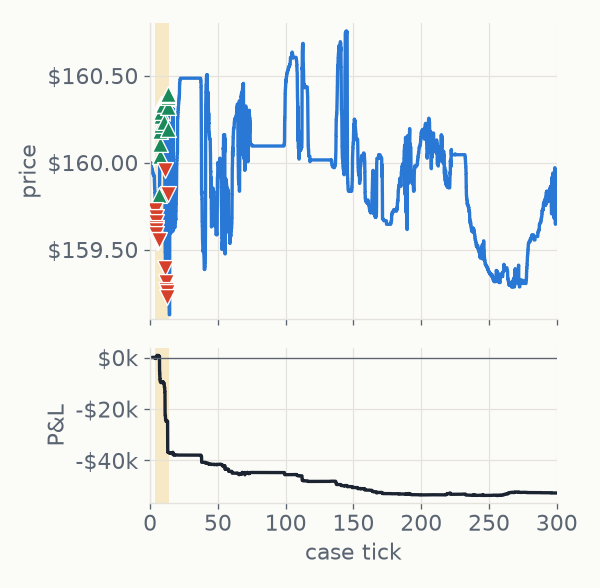
\includegraphics[width=\linewidth]{figures/J_CNR.png}\caption{CNR: $-\$53$k}\end{subfigure}\hfill
\begin{subfigure}{0.27\textwidth}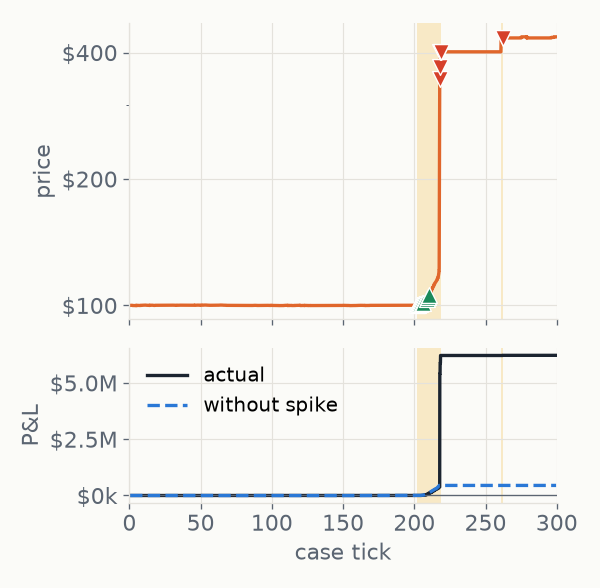
\includegraphics[width=\linewidth]{figures/J_RY.png}\caption{RY: $+\$6.22$M}\end{subfigure}\hfill
\begin{subfigure}{0.27\textwidth}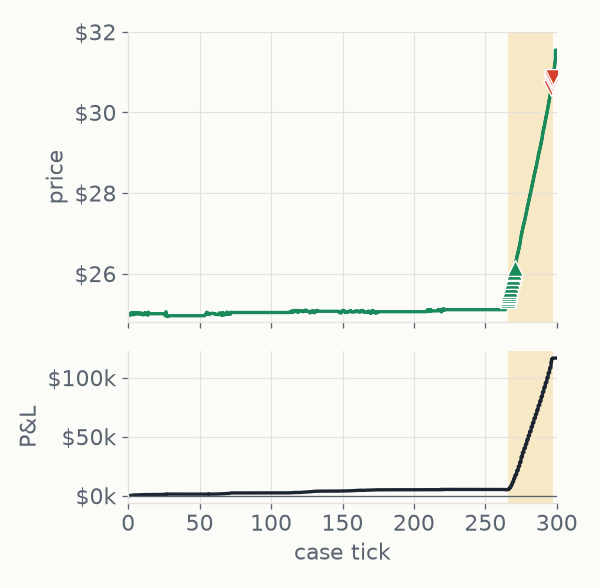
\includegraphics[width=\linewidth]{figures/J_AC.png}\caption{AC: $+\$117$k}\end{subfigure}
\caption{Price (top) and cumulative P\&L (bottom) per stock. Triangles: trend-engine buys and sells; shading: trend mode; dashed line (RY): P\&L without the tick-217 event.}
\label{fig:sec}
\end{figure}

\textbf{What the bot did, stock by stock.}
\begin{itemize}
  \item \textbf{CNR (ticks 3--13): false starts, then the learning rule worked.} The engine took three positions (short, long, short) that reversed almost immediately, losing \$36.7k.
        In the opening seconds CNR's book was thin, with spreads of 11 to 100 ticks and price jumps of 30--100 cents per tick, while the volatility estimate was still at its starting value.
        Noise therefore looked like a trend. Each loss raised CNR's entry bar by $1.4\times$, three losses in a row locked the engine out of CNR, and it never traded CNR directionally again.
        The account-level circuit breaker fired once, at tick 38, flattened everything and paused for eight seconds.
  \item \textbf{RY (ticks 200--218): the system working as designed.} At tick 200 the efficiency ratio jumped from 0 to 1.0, a straight-line move. At tick 201.6 the EMA gap had stayed above 12 ticks
        for 0.8\,s and the trend engine took over. Its first order was about 12{,}000 shares; by tick 210 it held 22{,}062 shares (88\% of the limit), bought between \$100.2 and \$105.5, and the
        wide trailing stop let it ride the drift to \$118. At tick 217 the RY book turned one-sided: the asks vanished and the bids jumped to \$346 and then \$402, following Group~12's activity.
        The engine sold the whole position into those bids in five orders over about four seconds, at an average of roughly \$383.
  \item \textbf{AC (ticks 265--296): a clean trend trade.} AC began a straight climb from \$25.1 to \$31.5. The engine entered at the start, held about 22{,}000 shares and closed in the end-of-case unwind.
\end{itemize}

\textbf{Why market making did not make money, even though prices mean-reverted.} This was the most instructive result. With a one-tick spread, a successful round trip earns about \$0.01 per share
plus the rebate. The inventory stop, however, cuts a losing position once it is down $\max(5\text{ ticks}, 3\sigma)$. With roughly $+1$ tick per winning trade and $-5$ ticks per stopped trade,
the market maker needs about five wins in every six trades just to break even. In this market prices moved in jumps of several cents rather than one-cent wiggles, so stops fired often
(86 times on CNR), and the orders that filled were disproportionately those a moving price ran through (adverse selection). Mean reversion in the \emph{price} is not the same thing as profitable
market making; the spread has to be wide relative to the size of the jumps.

\textbf{Size strategy: be big only when the evidence is strong or the risk is small.}
\begin{itemize}
  \item \textbf{Market-making quotes} were 5{,}000 shares a side in calm markets or healthy 2--6 tick spreads, 3{,}000 normally, half that when stressed, and 2{,}000 in thin books, so quote
        size falls exactly when the risk of being run over rises.
  \item \textbf{The inventory brake} uses $r = |\text{position}|/9{,}000$. The side that would add to the position is multiplied by $e^{-3r}$ and moved away from the market by
        $\operatorname{round}(4r^{1.5})$ ticks, and it is switched off entirely at $r \ge 0.85$ (7{,}650 shares), while the reducing side is enlarged by $(1+r)$. For example, holding
        4{,}500 shares ($r = 0.5$) cuts a 3{,}000-share adding quote to about 700 shares placed one tick further away, and raises the reducing quote to 4{,}500. This is a discrete version of the
        inventory skew in the Avellaneda--Stoikov market-making model.
  \item \textbf{Trend sizing} starts with 60\% of the available capacity and grows with the strength of the signal up to 95\% of the cap (about 22{,}000 shares), in orders of at most 5{,}000.
        The trend engine is the only part allowed to use most of the limit, because it only acts when the evidence is strong, and it carries a trailing stop.
  \item \textbf{Limits and unwinding.} On top of the 93\% pre-trade check, a safety net cuts the largest position immediately if the actual position ever passes 96\% of the limit; the \$40k
        drawdown breaker flattens the book; and about 20\,s before the close the bot stops adding risk and about 8\,s before it crosses to finish flat. After any trend exit the stock sells down in
        an ``exit'' mode with capped limit orders. Over the whole run the peak gross position was 23{,}088 and the peak net position 22{,}837, against a limit of 25{,}000.
\end{itemize}

\textbf{Our Python script and how to use it.} The trading code is listed in the Appendix (\code{algo2e\_strategy.py}). It needs Python 3 and the \code{requests} package. Start the RIT
client with the API enabled, note the API key and port, and run:
\begin{lstlisting}[basicstyle=\ttfamily\footnotesize, frame=single, columns=fullflexible, breaklines=true]
python algo2e_strategy.py <API_KEY> <PORT> [CASE_MINUTES]     # e.g. python algo2e_strategy.py abcde 15000 20
\end{lstlisting}
If started before the case begins, it waits until the case status is \code{ACTIVE}; without \code{CASE\_MINUTES} it learns the length of a tick from the case clock and scales its time windows
accordingly. Every parameter sits in one configuration block at the top of the file. Ctrl-C cancels all orders and flattens the book. While running it prints every fill, mode change and stop,
and once a second a status line per stock with its position, quotes and regime. It writes two logs: \code{logs/v3\_ticks\_*.csv}, one row per loop with prices, signals, positions, modes and P\&L
for every stock, and \code{logs/v3\_events\_*.csv}, every order, cancel, fill and decision with its reason. All numbers in this report come from these logs.
\code{dir.py} (trend engine only) and \code{mm.py} (market making only) are the same code with one engine disabled.

\textbf{Testing before the case.} During development we tested the bot against a fake exchange that reproduces RIT's order latency, position-reporting lag, rebates and fees, with eleven market scenarios. Re-running our development
script through all of them (90\,s each) gave: calm, mean-reverting and slow-grind markets between $-\$932$ and $+\$440$; trending, reversing and crashing markets $+\$41$k to $+\$124$k; spikes, sweeps
and one-sided order flow $+\$12$k to $+\$49$k; and a whipsaw market (short trends that reverse) $-\$44$k. Every run ended flat with peak gross at most 23{,}200 shares. The live result has the same
shape: break-even in calm markets, profits in trends, and the whipsaw case is the same failure mode as CNR's opening.

\textbf{A note on the following round.} In the next round our RIT client crashed, so we had cancelled the script and only started it after the round was under way (it first joined at tick 49 of 300).
It could not run the strategy as designed, and the late session ended with a small loss of \$3{,}427. We mention it for completeness only.

%==========================================================================================
\subsection*{(d) What was your P\&L?}

\textbf{The main strategy finished at \$6,288,771.} This is the server's net liquidation value. It equals the sum of the three stocks' P\&L to the cent, which is what we would expect if no fines were
charged. The two variants ran on separate accounts in the same market and are reported separately:

\vspace{-2pt}
\begin{table}[H]
\centering\footnotesize
\begin{tabular}{lrrrr}
\toprule
 & CNR & RY & AC & Total\\
\midrule
\code{algo2e\_fin.py} (market making + trend; main) & $-\$52{,}646$ & $\$6{,}224{,}827$ & $\$116{,}590$ & \textbf{\$6,288,771}\\
\code{dir.py} (trend engine only) & $-\$77{,}895$ & $\$6{,}238{,}173$ & $\$118{,}130$ & \$6,278,408\\
Market making only & $-\$28{,}719$ & $-\$6{,}147$ & $\$6{,}434$ & $-\$28{,}433$\\
\bottomrule
\end{tabular}
\end{table}
\vspace{-6pt}

\begin{figure}[!htb]
\centering
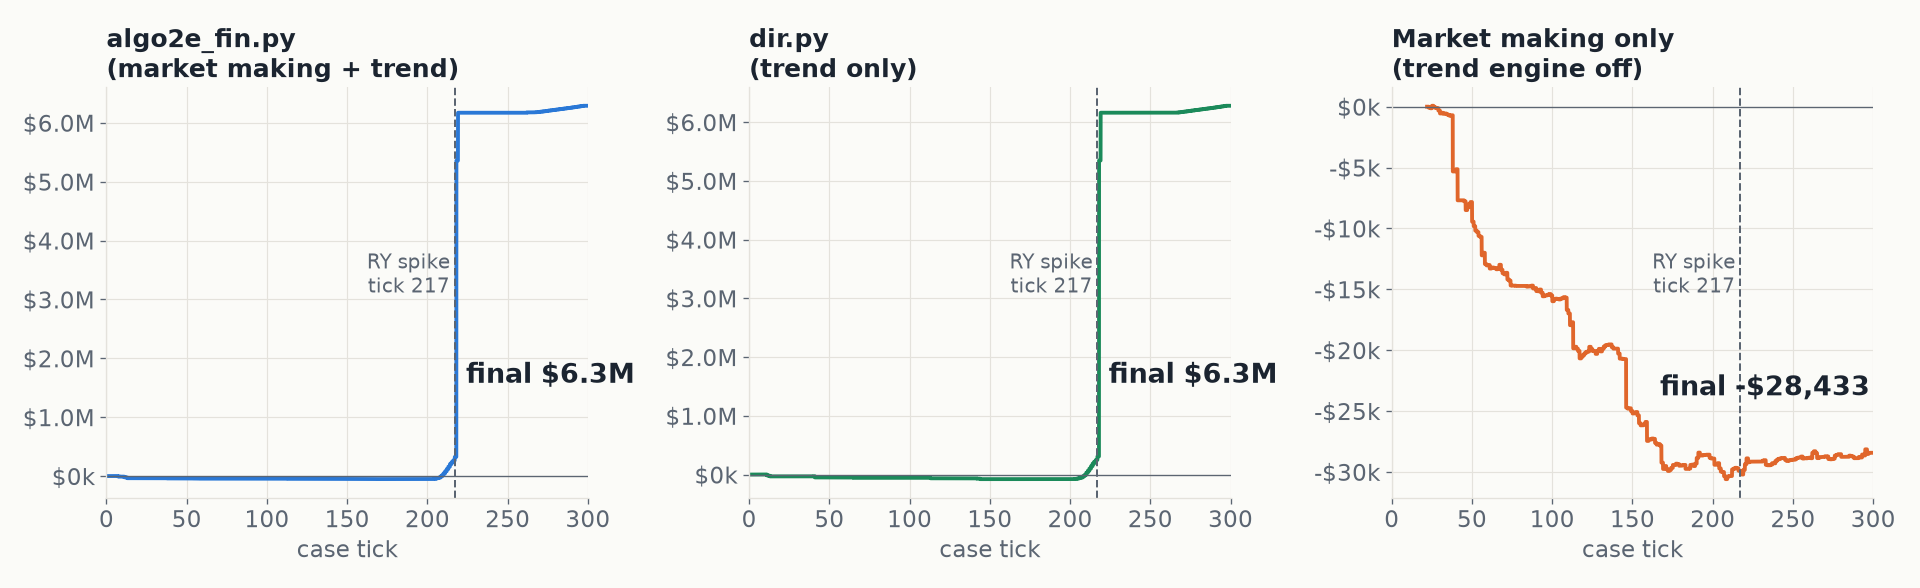
\includegraphics[width=0.8\textwidth]{figures/H3_total_pnl_three_algos.png}
\caption{Total P\&L through the case for the three builds; dashed line: the RY event at tick 217.}
\end{figure}
\vspace{-4pt}

\textbf{Where the money came from.} Splitting the main strategy's P\&L by the mode the bot was in shows a clear division of labour. The trend engine was in control for less than 7\% of the time on any
stock (about 2\% on CNR, 4\% on RY and 6\% on AC) and earned $+\$6.30$M net: $+\$5.78$M from selling RY into the dislocation, $+\$451$k from riding RY's drift before it, $+\$112$k on AC, less \$36k on
CNR's early false starts. Market making, active the rest of the time, finished at about $-\$15$k. Running three builds side by side in the same market makes this a controlled comparison: the same trend
engine produced almost the same result with or without market making, while market making alone lost money. \code{dir.py}'s faster entries (8-tick instead of 12-tick threshold) lost more on CNR,
which illustrates the trade-off between catching a move early and reacting to noise.

\textbf{With and without the RY event.} About 92\% of the profit came from one event, so we also measured what the strategy earned on its own terms. Re-valuing the RY exit at the last normal bid before
the book broke (\$121.08), with everything else unchanged, gives about \textbf{\$511k}, and between \$244k and \$559k for exit prices from \$109 to \$123. This still includes the RY drift that preceded the
event, so it is the optimistic reading; ticks 0--199 on their own were a loss of about \$52k.

\textbf{What the mean-reversion tilt would have added.} Replaying the logged Bollinger z-scores and regime labels, and holding the position the tilt would have targeted, gives about $+\$37$k at 8{,}000
shares and $+\$56$k at 12{,}000 before trading costs, and roughly $+\$5$k to $+\$20$k after them. Almost all of it falls before tick 200, because the tilt switches itself off when a stock is in TREND,
so it would not have been short RY into the event. At under 1\% of the total, this supports our decision to leave it off.

\textbf{How we read the result.} We did not predict the RY event, and we do not claim to have. What the system did was put the right position on by rule before the event: regime detection moved RY
into trend mode within about one case tick of the drift starting, the trend engine sized up to 88\% of the limit, and the volatility-scaled trailing stop kept the position on until the book broke.
The position stayed within limits for the whole case and no fines were charged. The run also showed the two changes we would make first: a warm-up period before the trend engine is allowed to trade,
and fee-aware quoting restricted to stocks where resting orders earn a rebate.
 inside your document.
% Needs in the preamble: amsmath, booktabs, tabularx, graphicx, float, caption, subcaption, xcolor, listings, enumitem
\providecommand{\code}[1]{\texttt{#1}}
\section*{RIT ALGO2e: Strategy Report}
\addcontentsline{toc}{section}{RIT ALGO2e: Strategy Report}
Main strategy: \code{algo2e\_fin.py} (trading code in Appendix~\ref{app:code}).


%==========================================================================================
\subsection*{(a) What was your strategy going in?}

\textbf{The problem.} ALGO2e is a liquidity-provision case: three stocks (CNR $\approx$\$160, RY $\approx$\$100, AC $\approx$\$25), a 25{,}000-share gross and net
limit with fines for breaches, and a fee schedule that pays a rebate for resting orders on two of the three stocks. Market making is the natural way to earn money
here: quote a bid and an ask, collect the spread and the rebate, and keep inventory near zero. It is also the natural way to lose money, because in a trending market
a market maker keeps buying a falling price (or selling a rising one) and ends up holding a large position against the move. We did not know in advance which kind
of market the case would produce. Our working guess was that prices would mostly mean-revert around an anchor, with the possibility of trends or shocks injected during
the case. The strategy therefore had to make money in a calm market, survive a trending one, and switch between the two without anyone touching it.

\textbf{The design: a regime-switching system with three parts.}
\begin{enumerate}
  \item \textbf{Market maker (base income in calm markets).} Passive quotes on every stock, sized according to how volatile the stock currently is, with an
        inventory brake that makes it progressively harder to add to a position and easier to reduce it.
  \item \textbf{Trend engine (insurance against our guess being wrong).} When a stock starts moving steadily in one direction, quoting on that stock stops and
        the engine takes a large position \emph{with} the move, held with a trailing stop that is scaled to the stock's volatility.
  \item \textbf{Risk layer (overrides both).} Only limit orders are used, every order is checked against worst-case exposure before it is sent, and an account-level
        circuit breaker and end-of-case unwind sit on top. Our explicit objective was profit with \emph{zero fines}.
\end{enumerate}
Each stock is handled every pass of the loop (up to 40 times a second) in a fixed order of precedence: end-of-case unwind or circuit breaker first, then the trend engine,
then market-making loss controls, and only then new quotes. The first rule that applies wins, so safety always takes priority over making money.

\textbf{How the bot knows which regime it is in.} For every stock the bot keeps a few simple, robust measurements:
the \emph{EMA gap}, the difference between a fast (1\,s) and a slow (8\,s) exponential moving average of the mid-price, measured in ticks, which says how far the
price has run from its recent past; the \emph{Kaufman efficiency ratio} over 10\,s, $|\text{net move}|/\text{total path}$, which is close to 1 when the price moves in a
straight line and close to 0 when it goes back and forth; the width of its \emph{Bollinger bands} relative to their own 2-minute baseline, which classifies the stock as
calm, normal or stressed; a short-term \emph{volatility} estimate; and a \emph{t-statistic} of the drift over 20 case ticks for slow, grinding trends. A stock is labelled
TREND when the efficiency ratio is at least 0.45 and the move is at least 12 ticks, and it keeps that label until the ratio falls below 0.33. This hysteresis stops the label
from flickering on the boundary. Importantly, the label alone never triggers a trade. The trend engine also requires the EMA gap to exceed $\max(12\text{ ticks}, 5\sigma)$,
the spread to be at most 6 ticks, and the signal to persist for 0.8\,s. Because the thresholds are expressed in units of the stock's own volatility, the same rules work for a
\$25 stock and a \$160 stock, and a noisy stock needs a bigger move before the engine believes it.

\textbf{What we decided against.} We also built a directional mean-reversion tilt: instead of steering inventory to zero, it targets a long position when the price is low in
its Bollinger band and a short one when it is high (up to 8{,}000--12{,}000 shares). In testing it did worse than plain inventory-to-zero market making, because it is holding
inventory against the move at exactly the moment a breakout starts. It was switched off for the graded run (\code{MR\_MAX\_INV = 0}). Several other rules came from our practice
sessions: market orders into a thin AC book lost tens of thousands of dollars in a second, so every aggressive order is a limit order capped within 2\% of fair value; and a
bot that reads its own resting quotes as ``the market'' keeps outbidding itself, so the bot strips its own orders from the book before computing any price.

%==========================================================================================
\subsection*{(b) What changes did you make to handle multiple securities and fees/rebates?}

\textbf{Nothing about the securities is hard-coded.} At start-up the bot reads \code{/securities} for the list of tradeable tickers and each ticker's tick size, taker fee
and maker rebate, and \code{/limits} for the gross and net limits and the fine schedule. Its own caps are derived from these values, so the same script runs unchanged on
two, three or ten securities and on a different limit.

\textbf{Each stock thinks for itself; all stocks share one risk budget.} Every stock has its own signals, regime label, mode (market making, trend, or exiting a trend),
stops, loss pauses and a learned entry threshold that rises after losing trend trades on that stock. What the stocks cannot each have is their own limit, because the
25{,}000-share limit is shared. We handled this in four ways:
\begin{itemize}
  \item \textbf{Aggregate worst-case check.} Before any order is sent, the bot assumes that every resting order, every order still in flight and the new order all fill at once,
        summed across all stocks, and requires gross and net exposure to stay below 93\% of the limit (23{,}250 shares). If the order does not fit, it is shrunk by 40\% at a time
        and dropped if it still does not fit.
  \item \textbf{Capacity allocation.} The trend engine's maximum size on one stock is $0.95\times$ the cap minus whatever is held in the other stocks. When RY's trend started the
        other books were almost flat, so RY could take about 22{,}000 shares; had AC been trending at the same time, RY would have received only what was left.
  \item \textbf{Per-stock inventory caps.} Market-making inventory is limited to 9{,}000 shares per stock, so one stock cannot absorb the whole budget through passive fills.
  \item \textbf{Priority when room is tight.} Aggressive orders (stops, trend trades, unwind) are processed first, then the quotes of the stock with the healthiest wide spread,
        which is the most profitable to quote, then the remaining quotes.
\end{itemize}
Order books for all stocks are fetched in parallel so that adding a stock does not slow the loop. Because RIT confirms orders and updates positions with a delay, the bot keeps its own
registry of orders: a just-sent order counts as live before RIT lists it, and an order that has disappeared still counts toward exposure for a second, until the position catches up.

\textbf{Fees and rebates.} The useful way to read the fee schedule is as a fraction of the one-tick (\$0.01) spread, because that is all a market maker earns per share:

\vspace{-2pt}
\begin{table}[H]
\centering\footnotesize
\begin{tabular}{lrrl}
\toprule
 & Maker rebate (resting) & Taker fee (crossing) & What it means for us\\
\midrule
CNR & $+\$0.0023$ (23\% of a tick) & \$0.0027 (27\% of a tick) & rest; crossing costs $>$\,\textonequarter\ of the spread\\
AC  & $+\$0.0011$ (11\%) & \$0.0015 (15\%) & rest\\
RY  & $-\$0.0020$ (resting \emph{pays} 20\%) & $-\$0.0014$ (crossing \emph{earns} 14\%) & resting costs; crossing is cheap\\
\bottomrule
\end{tabular}
\end{table}
\vspace{-4pt}
A 1{,}000-share round trip on CNR earns \$10 of spread plus \$4.60 of rebates if both sides rest, but crossing both sides would cost the \$10 spread plus \$5.40 in fees. That asymmetry
drove three choices. First, \textbf{passive-first execution}: market making only rests orders, and we cross the spread only when we must (stops, trend entries and exits, the final unwind),
always with capped limit orders. Second, \textbf{size where the economics are best}: full size (5{,}000 shares a side) is quoted only when the market is calm or the spread is a
``healthy'' 2--6 ticks, where spread plus rebate can pay for the inventory risk; on a 2-tick spread we step inside only on the side that reduces our position. Third,
\textbf{RY is different}: resting there costs money, so market making on RY is structurally weak, while our RY trend trades were executed aggressively, which is the cheaper side on that stock.
In this version the fee schedule shaped the design rather than entering the quoting formula itself; making quotes explicitly fee-aware, for example not resting on RY at all, is the
first change we would make.

%==========================================================================================
\subsection*{(c) What happened during the simulation? What was your size strategy?}

\textbf{The market we got.} For the first 200 case ticks all three prices behaved like mean-reverting series. Their 10-tick variance ratios were 0.19--0.26 (a random walk scores 1),
and consecutive returns were negatively correlated ($-0.21$ to $-0.33$), so our working assumption held for two-thirds of the case. After tick 200 the picture changed: RY broke out,
AC trended steadily, and CNR stayed inside its band to the end (Figure~\ref{fig:sec}).

\begin{figure}[!htb]
\centering\hspace*{0.05\textwidth}
\begin{subfigure}{0.27\textwidth}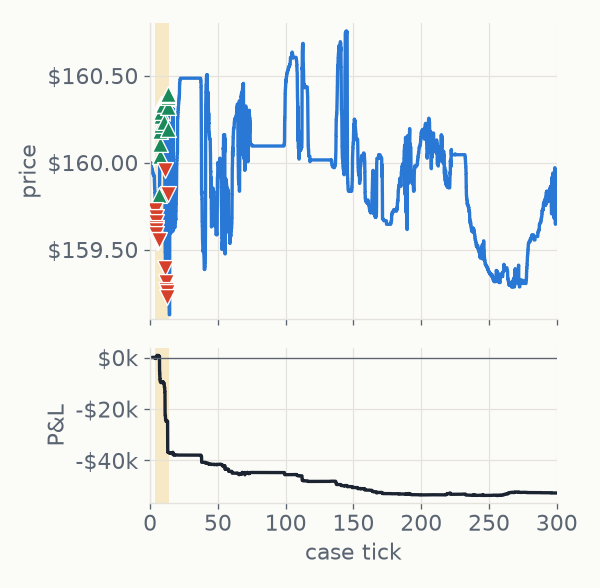
\includegraphics[width=\linewidth]{figures/J_CNR.png}\caption{CNR: $-\$53$k}\end{subfigure}\hfill
\begin{subfigure}{0.27\textwidth}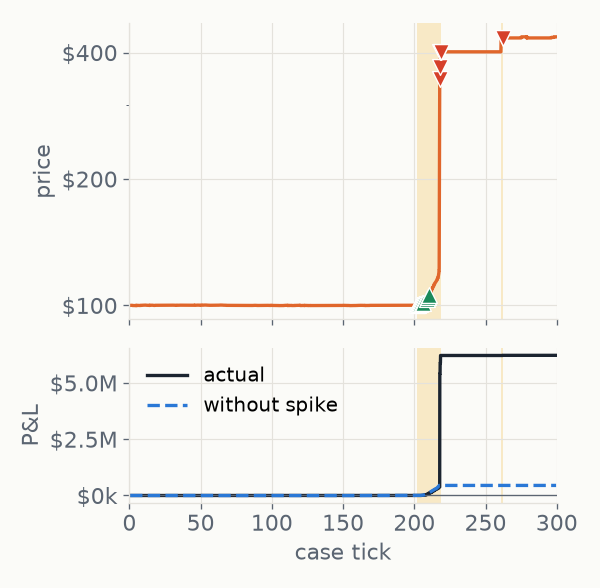
\includegraphics[width=\linewidth]{figures/J_RY.png}\caption{RY: $+\$6.22$M}\end{subfigure}\hfill
\begin{subfigure}{0.27\textwidth}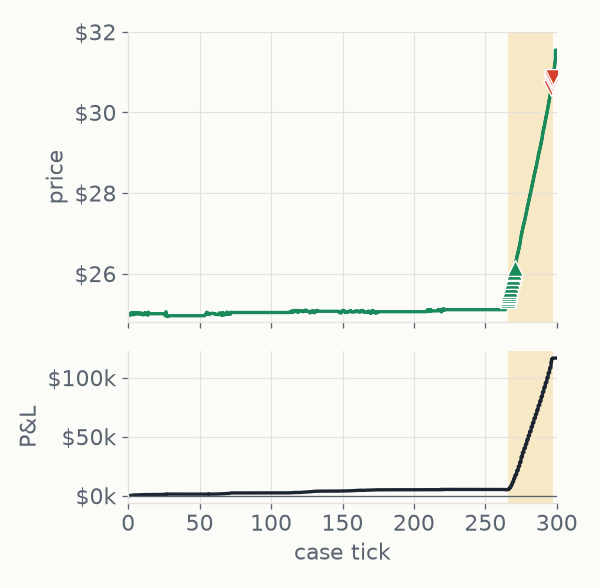
\includegraphics[width=\linewidth]{figures/J_AC.png}\caption{AC: $+\$117$k}\end{subfigure}
\caption{Price (top) and cumulative P\&L (bottom) per stock. Triangles: trend-engine buys and sells; shading: trend mode; dashed line (RY): P\&L without the tick-217 event.}
\label{fig:sec}
\end{figure}

\textbf{What the bot did, stock by stock.}
\begin{itemize}
  \item \textbf{CNR (ticks 3--13): false starts, then the learning rule worked.} The engine took three positions (short, long, short) that reversed almost immediately, losing \$36.7k.
        In the opening seconds CNR's book was thin, with spreads of 11 to 100 ticks and price jumps of 30--100 cents per tick, while the volatility estimate was still at its starting value.
        Noise therefore looked like a trend. Each loss raised CNR's entry bar by $1.4\times$, three losses in a row locked the engine out of CNR, and it never traded CNR directionally again.
        The account-level circuit breaker fired once, at tick 38, flattened everything and paused for eight seconds.
  \item \textbf{RY (ticks 200--218): the system working as designed.} At tick 200 the efficiency ratio jumped from 0 to 1.0, a straight-line move. At tick 201.6 the EMA gap had stayed above 12 ticks
        for 0.8\,s and the trend engine took over. Its first order was about 12{,}000 shares; by tick 210 it held 22{,}062 shares (88\% of the limit), bought between \$100.2 and \$105.5, and the
        wide trailing stop let it ride the drift to \$118. At tick 217 the RY book turned one-sided: the asks vanished and the bids jumped to \$346 and then \$402, following Group~12's activity.
        The engine sold the whole position into those bids in five orders over about four seconds, at an average of roughly \$383.
  \item \textbf{AC (ticks 265--296): a clean trend trade.} AC began a straight climb from \$25.1 to \$31.5. The engine entered at the start, held about 22{,}000 shares and closed in the end-of-case unwind.
\end{itemize}

\textbf{Why market making did not make money, even though prices mean-reverted.} This was the most instructive result. With a one-tick spread, a successful round trip earns about \$0.01 per share
plus the rebate. The inventory stop, however, cuts a losing position once it is down $\max(5\text{ ticks}, 3\sigma)$. With roughly $+1$ tick per winning trade and $-5$ ticks per stopped trade,
the market maker needs about five wins in every six trades just to break even. In this market prices moved in jumps of several cents rather than one-cent wiggles, so stops fired often
(86 times on CNR), and the orders that filled were disproportionately those a moving price ran through (adverse selection). Mean reversion in the \emph{price} is not the same thing as profitable
market making; the spread has to be wide relative to the size of the jumps.

\textbf{Size strategy: be big only when the evidence is strong or the risk is small.}
\begin{itemize}
  \item \textbf{Market-making quotes} were 5{,}000 shares a side in calm markets or healthy 2--6 tick spreads, 3{,}000 normally, half that when stressed, and 2{,}000 in thin books, so quote
        size falls exactly when the risk of being run over rises.
  \item \textbf{The inventory brake} uses $r = |\text{position}|/9{,}000$. The side that would add to the position is multiplied by $e^{-3r}$ and moved away from the market by
        $\operatorname{round}(4r^{1.5})$ ticks, and it is switched off entirely at $r \ge 0.85$ (7{,}650 shares), while the reducing side is enlarged by $(1+r)$. For example, holding
        4{,}500 shares ($r = 0.5$) cuts a 3{,}000-share adding quote to about 700 shares placed one tick further away, and raises the reducing quote to 4{,}500. This is a discrete version of the
        inventory skew in the Avellaneda--Stoikov market-making model.
  \item \textbf{Trend sizing} starts with 60\% of the available capacity and grows with the strength of the signal up to 95\% of the cap (about 22{,}000 shares), in orders of at most 5{,}000.
        The trend engine is the only part allowed to use most of the limit, because it only acts when the evidence is strong, and it carries a trailing stop.
  \item \textbf{Limits and unwinding.} On top of the 93\% pre-trade check, a safety net cuts the largest position immediately if the actual position ever passes 96\% of the limit; the \$40k
        drawdown breaker flattens the book; and about 20\,s before the close the bot stops adding risk and about 8\,s before it crosses to finish flat. After any trend exit the stock sells down in
        an ``exit'' mode with capped limit orders. Over the whole run the peak gross position was 23{,}088 and the peak net position 22{,}837, against a limit of 25{,}000.
\end{itemize}

\textbf{Our Python script and how to use it.} The trading code is listed in the Appendix (\code{algo2e\_strategy.py}). It needs Python 3 and the \code{requests} package. Start the RIT
client with the API enabled, note the API key and port, and run:
\begin{lstlisting}[basicstyle=\ttfamily\footnotesize, frame=single, columns=fullflexible, breaklines=true]
python algo2e_strategy.py <API_KEY> <PORT> [CASE_MINUTES]     # e.g. python algo2e_strategy.py abcde 15000 20
\end{lstlisting}
If started before the case begins, it waits until the case status is \code{ACTIVE}; without \code{CASE\_MINUTES} it learns the length of a tick from the case clock and scales its time windows
accordingly. Every parameter sits in one configuration block at the top of the file. Ctrl-C cancels all orders and flattens the book. While running it prints every fill, mode change and stop,
and once a second a status line per stock with its position, quotes and regime. It writes two logs: \code{logs/v3\_ticks\_*.csv}, one row per loop with prices, signals, positions, modes and P\&L
for every stock, and \code{logs/v3\_events\_*.csv}, every order, cancel, fill and decision with its reason. All numbers in this report come from these logs.
\code{dir.py} (trend engine only) and \code{mm.py} (market making only) are the same code with one engine disabled.

\textbf{Testing before the case.} During development we tested the bot against a fake exchange that reproduces RIT's order latency, position-reporting lag, rebates and fees, with eleven market scenarios. Re-running our development
script through all of them (90\,s each) gave: calm, mean-reverting and slow-grind markets between $-\$932$ and $+\$440$; trending, reversing and crashing markets $+\$41$k to $+\$124$k; spikes, sweeps
and one-sided order flow $+\$12$k to $+\$49$k; and a whipsaw market (short trends that reverse) $-\$44$k. Every run ended flat with peak gross at most 23{,}200 shares. The live result has the same
shape: break-even in calm markets, profits in trends, and the whipsaw case is the same failure mode as CNR's opening.

\textbf{A note on the following round.} In the next round our RIT client crashed, so we had cancelled the script and only started it after the round was under way (it first joined at tick 49 of 300).
It could not run the strategy as designed, and the late session ended with a small loss of \$3{,}427. We mention it for completeness only.

%==========================================================================================
\subsection*{(d) What was your P\&L?}

\textbf{The main strategy finished at \$6,288,771.} This is the server's net liquidation value. It equals the sum of the three stocks' P\&L to the cent, which is what we would expect if no fines were
charged. The two variants ran on separate accounts in the same market and are reported separately:

\vspace{-2pt}
\begin{table}[H]
\centering\footnotesize
\begin{tabular}{lrrrr}
\toprule
 & CNR & RY & AC & Total\\
\midrule
\code{algo2e\_fin.py} (market making + trend; main) & $-\$52{,}646$ & $\$6{,}224{,}827$ & $\$116{,}590$ & \textbf{\$6,288,771}\\
\code{dir.py} (trend engine only) & $-\$77{,}895$ & $\$6{,}238{,}173$ & $\$118{,}130$ & \$6,278,408\\
Market making only & $-\$28{,}719$ & $-\$6{,}147$ & $\$6{,}434$ & $-\$28{,}433$\\
\bottomrule
\end{tabular}
\end{table}
\vspace{-6pt}

\begin{figure}[!htb]
\centering
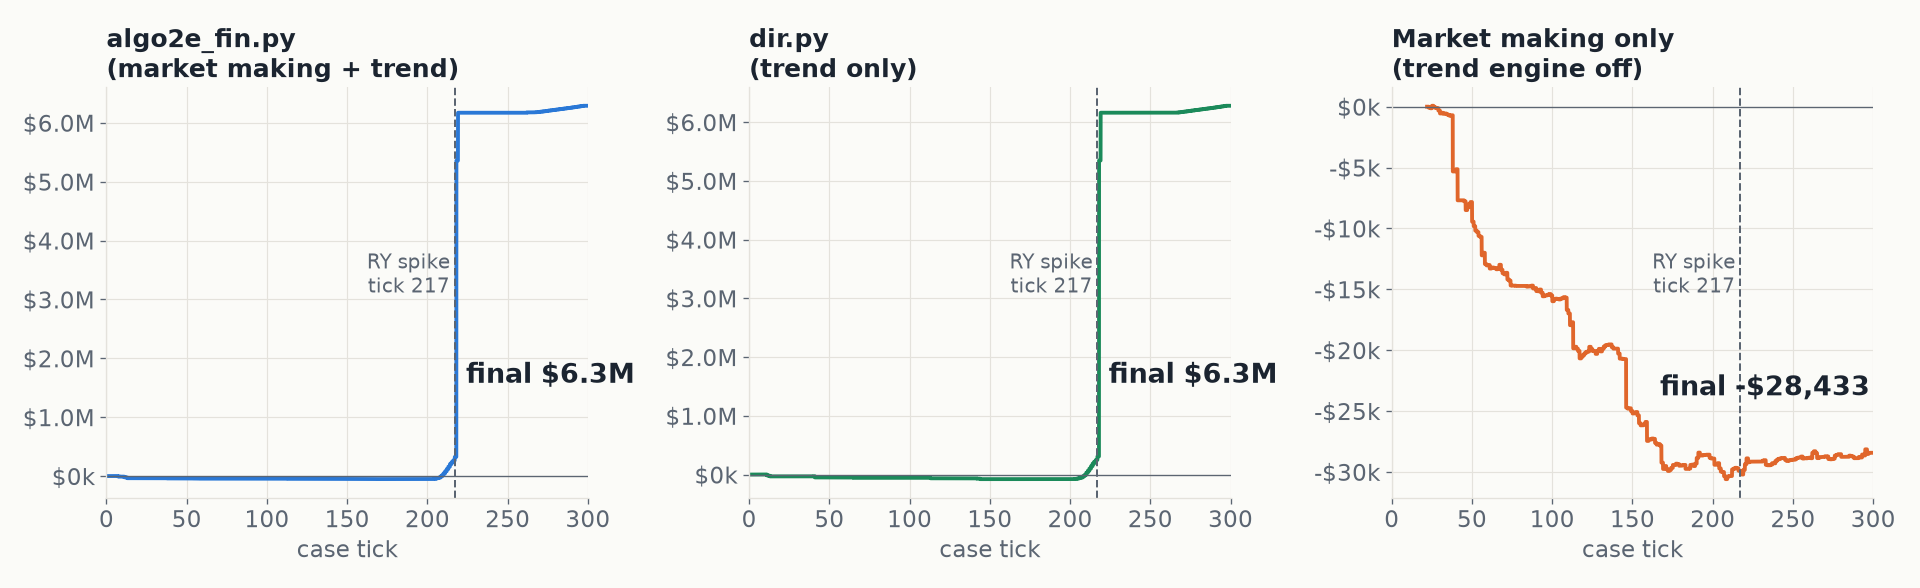
\includegraphics[width=0.8\textwidth]{figures/H3_total_pnl_three_algos.png}
\caption{Total P\&L through the case for the three builds; dashed line: the RY event at tick 217.}
\end{figure}
\vspace{-4pt}

\textbf{Where the money came from.} Splitting the main strategy's P\&L by the mode the bot was in shows a clear division of labour. The trend engine was in control for less than 7\% of the time on any
stock (about 2\% on CNR, 4\% on RY and 6\% on AC) and earned $+\$6.30$M net: $+\$5.78$M from selling RY into the dislocation, $+\$451$k from riding RY's drift before it, $+\$112$k on AC, less \$36k on
CNR's early false starts. Market making, active the rest of the time, finished at about $-\$15$k. Running three builds side by side in the same market makes this a controlled comparison: the same trend
engine produced almost the same result with or without market making, while market making alone lost money. \code{dir.py}'s faster entries (8-tick instead of 12-tick threshold) lost more on CNR,
which illustrates the trade-off between catching a move early and reacting to noise.

\textbf{With and without the RY event.} About 92\% of the profit came from one event, so we also measured what the strategy earned on its own terms. Re-valuing the RY exit at the last normal bid before
the book broke (\$121.08), with everything else unchanged, gives about \textbf{\$511k}, and between \$244k and \$559k for exit prices from \$109 to \$123. This still includes the RY drift that preceded the
event, so it is the optimistic reading; ticks 0--199 on their own were a loss of about \$52k.

\textbf{What the mean-reversion tilt would have added.} Replaying the logged Bollinger z-scores and regime labels, and holding the position the tilt would have targeted, gives about $+\$37$k at 8{,}000
shares and $+\$56$k at 12{,}000 before trading costs, and roughly $+\$5$k to $+\$20$k after them. Almost all of it falls before tick 200, because the tilt switches itself off when a stock is in TREND,
so it would not have been short RY into the event. At under 1\% of the total, this supports our decision to leave it off.

\textbf{How we read the result.} We did not predict the RY event, and we do not claim to have. What the system did was put the right position on by rule before the event: regime detection moved RY
into trend mode within about one case tick of the drift starting, the trend engine sized up to 88\% of the limit, and the volatility-scaled trailing stop kept the position on until the book broke.
The position stayed within limits for the whole case and no fines were charged. The run also showed the two changes we would make first: a warm-up period before the trend engine is allowed to trade,
and fee-aware quoting restricted to stocks where resting orders earn a rebate.
 inside your document.
% Needs in the preamble: amsmath, booktabs, tabularx, graphicx, float, caption, subcaption, xcolor, listings, enumitem
\providecommand{\code}[1]{\texttt{#1}}
\section*{RIT ALGO2e: Strategy Report}
\addcontentsline{toc}{section}{RIT ALGO2e: Strategy Report}
Main strategy: \code{algo2e\_fin.py} (trading code in Appendix~\ref{app:code}).


%==========================================================================================
\subsection*{(a) What was your strategy going in?}

\textbf{The problem.} ALGO2e is a liquidity-provision case: three stocks (CNR $\approx$\$160, RY $\approx$\$100, AC $\approx$\$25), a 25{,}000-share gross and net
limit with fines for breaches, and a fee schedule that pays a rebate for resting orders on two of the three stocks. Market making is the natural way to earn money
here: quote a bid and an ask, collect the spread and the rebate, and keep inventory near zero. It is also the natural way to lose money, because in a trending market
a market maker keeps buying a falling price (or selling a rising one) and ends up holding a large position against the move. We did not know in advance which kind
of market the case would produce. Our working guess was that prices would mostly mean-revert around an anchor, with the possibility of trends or shocks injected during
the case. The strategy therefore had to make money in a calm market, survive a trending one, and switch between the two without anyone touching it.

\textbf{The design: a regime-switching system with three parts.}
\begin{enumerate}
  \item \textbf{Market maker (base income in calm markets).} Passive quotes on every stock, sized according to how volatile the stock currently is, with an
        inventory brake that makes it progressively harder to add to a position and easier to reduce it.
  \item \textbf{Trend engine (insurance against our guess being wrong).} When a stock starts moving steadily in one direction, quoting on that stock stops and
        the engine takes a large position \emph{with} the move, held with a trailing stop that is scaled to the stock's volatility.
  \item \textbf{Risk layer (overrides both).} Only limit orders are used, every order is checked against worst-case exposure before it is sent, and an account-level
        circuit breaker and end-of-case unwind sit on top. Our explicit objective was profit with \emph{zero fines}.
\end{enumerate}
Each stock is handled every pass of the loop (up to 40 times a second) in a fixed order of precedence: end-of-case unwind or circuit breaker first, then the trend engine,
then market-making loss controls, and only then new quotes. The first rule that applies wins, so safety always takes priority over making money.

\textbf{How the bot knows which regime it is in.} For every stock the bot keeps a few simple, robust measurements:
the \emph{EMA gap}, the difference between a fast (1\,s) and a slow (8\,s) exponential moving average of the mid-price, measured in ticks, which says how far the
price has run from its recent past; the \emph{Kaufman efficiency ratio} over 10\,s, $|\text{net move}|/\text{total path}$, which is close to 1 when the price moves in a
straight line and close to 0 when it goes back and forth; the width of its \emph{Bollinger bands} relative to their own 2-minute baseline, which classifies the stock as
calm, normal or stressed; a short-term \emph{volatility} estimate; and a \emph{t-statistic} of the drift over 20 case ticks for slow, grinding trends. A stock is labelled
TREND when the efficiency ratio is at least 0.45 and the move is at least 12 ticks, and it keeps that label until the ratio falls below 0.33. This hysteresis stops the label
from flickering on the boundary. Importantly, the label alone never triggers a trade. The trend engine also requires the EMA gap to exceed $\max(12\text{ ticks}, 5\sigma)$,
the spread to be at most 6 ticks, and the signal to persist for 0.8\,s. Because the thresholds are expressed in units of the stock's own volatility, the same rules work for a
\$25 stock and a \$160 stock, and a noisy stock needs a bigger move before the engine believes it.

\textbf{What we decided against.} We also built a directional mean-reversion tilt: instead of steering inventory to zero, it targets a long position when the price is low in
its Bollinger band and a short one when it is high (up to 8{,}000--12{,}000 shares). In testing it did worse than plain inventory-to-zero market making, because it is holding
inventory against the move at exactly the moment a breakout starts. It was switched off for the graded run (\code{MR\_MAX\_INV = 0}). Several other rules came from our practice
sessions: market orders into a thin AC book lost tens of thousands of dollars in a second, so every aggressive order is a limit order capped within 2\% of fair value; and a
bot that reads its own resting quotes as ``the market'' keeps outbidding itself, so the bot strips its own orders from the book before computing any price.

%==========================================================================================
\subsection*{(b) What changes did you make to handle multiple securities and fees/rebates?}

\textbf{Nothing about the securities is hard-coded.} At start-up the bot reads \code{/securities} for the list of tradeable tickers and each ticker's tick size, taker fee
and maker rebate, and \code{/limits} for the gross and net limits and the fine schedule. Its own caps are derived from these values, so the same script runs unchanged on
two, three or ten securities and on a different limit.

\textbf{Each stock thinks for itself; all stocks share one risk budget.} Every stock has its own signals, regime label, mode (market making, trend, or exiting a trend),
stops, loss pauses and a learned entry threshold that rises after losing trend trades on that stock. What the stocks cannot each have is their own limit, because the
25{,}000-share limit is shared. We handled this in four ways:
\begin{itemize}
  \item \textbf{Aggregate worst-case check.} Before any order is sent, the bot assumes that every resting order, every order still in flight and the new order all fill at once,
        summed across all stocks, and requires gross and net exposure to stay below 93\% of the limit (23{,}250 shares). If the order does not fit, it is shrunk by 40\% at a time
        and dropped if it still does not fit.
  \item \textbf{Capacity allocation.} The trend engine's maximum size on one stock is $0.95\times$ the cap minus whatever is held in the other stocks. When RY's trend started the
        other books were almost flat, so RY could take about 22{,}000 shares; had AC been trending at the same time, RY would have received only what was left.
  \item \textbf{Per-stock inventory caps.} Market-making inventory is limited to 9{,}000 shares per stock, so one stock cannot absorb the whole budget through passive fills.
  \item \textbf{Priority when room is tight.} Aggressive orders (stops, trend trades, unwind) are processed first, then the quotes of the stock with the healthiest wide spread,
        which is the most profitable to quote, then the remaining quotes.
\end{itemize}
Order books for all stocks are fetched in parallel so that adding a stock does not slow the loop. Because RIT confirms orders and updates positions with a delay, the bot keeps its own
registry of orders: a just-sent order counts as live before RIT lists it, and an order that has disappeared still counts toward exposure for a second, until the position catches up.

\textbf{Fees and rebates.} The useful way to read the fee schedule is as a fraction of the one-tick (\$0.01) spread, because that is all a market maker earns per share:

\vspace{-2pt}
\begin{table}[H]
\centering\footnotesize
\begin{tabular}{lrrl}
\toprule
 & Maker rebate (resting) & Taker fee (crossing) & What it means for us\\
\midrule
CNR & $+\$0.0023$ (23\% of a tick) & \$0.0027 (27\% of a tick) & rest; crossing costs $>$\,\textonequarter\ of the spread\\
AC  & $+\$0.0011$ (11\%) & \$0.0015 (15\%) & rest\\
RY  & $-\$0.0020$ (resting \emph{pays} 20\%) & $-\$0.0014$ (crossing \emph{earns} 14\%) & resting costs; crossing is cheap\\
\bottomrule
\end{tabular}
\end{table}
\vspace{-4pt}
A 1{,}000-share round trip on CNR earns \$10 of spread plus \$4.60 of rebates if both sides rest, but crossing both sides would cost the \$10 spread plus \$5.40 in fees. That asymmetry
drove three choices. First, \textbf{passive-first execution}: market making only rests orders, and we cross the spread only when we must (stops, trend entries and exits, the final unwind),
always with capped limit orders. Second, \textbf{size where the economics are best}: full size (5{,}000 shares a side) is quoted only when the market is calm or the spread is a
``healthy'' 2--6 ticks, where spread plus rebate can pay for the inventory risk; on a 2-tick spread we step inside only on the side that reduces our position. Third,
\textbf{RY is different}: resting there costs money, so market making on RY is structurally weak, while our RY trend trades were executed aggressively, which is the cheaper side on that stock.
In this version the fee schedule shaped the design rather than entering the quoting formula itself; making quotes explicitly fee-aware, for example not resting on RY at all, is the
first change we would make.

%==========================================================================================
\subsection*{(c) What happened during the simulation? What was your size strategy?}

\textbf{The market we got.} For the first 200 case ticks all three prices behaved like mean-reverting series. Their 10-tick variance ratios were 0.19--0.26 (a random walk scores 1),
and consecutive returns were negatively correlated ($-0.21$ to $-0.33$), so our working assumption held for two-thirds of the case. After tick 200 the picture changed: RY broke out,
AC trended steadily, and CNR stayed inside its band to the end (Figure~\ref{fig:sec}).

\begin{figure}[!htb]
\centering\hspace*{0.05\textwidth}
\begin{subfigure}{0.27\textwidth}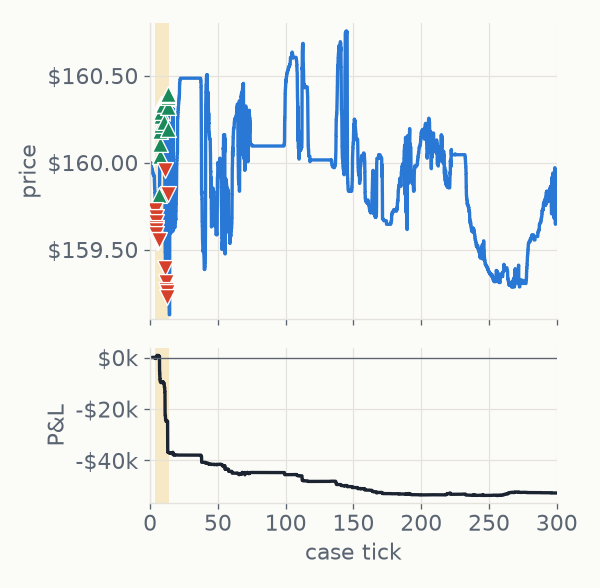
\includegraphics[width=\linewidth]{figures/J_CNR.png}\caption{CNR: $-\$53$k}\end{subfigure}\hfill
\begin{subfigure}{0.27\textwidth}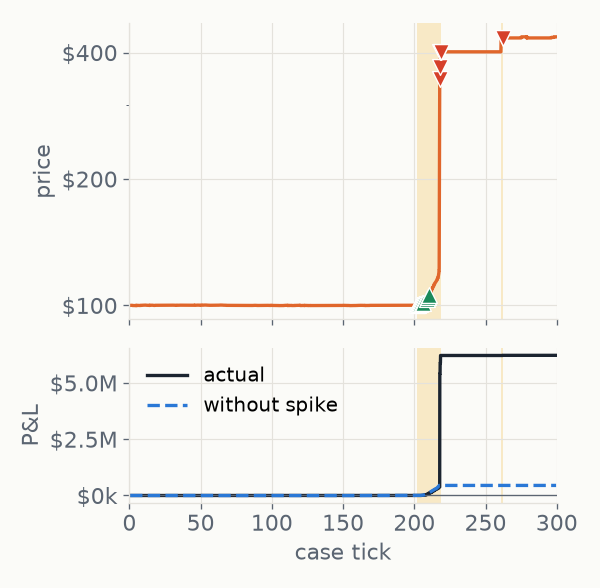
\includegraphics[width=\linewidth]{figures/J_RY.png}\caption{RY: $+\$6.22$M}\end{subfigure}\hfill
\begin{subfigure}{0.27\textwidth}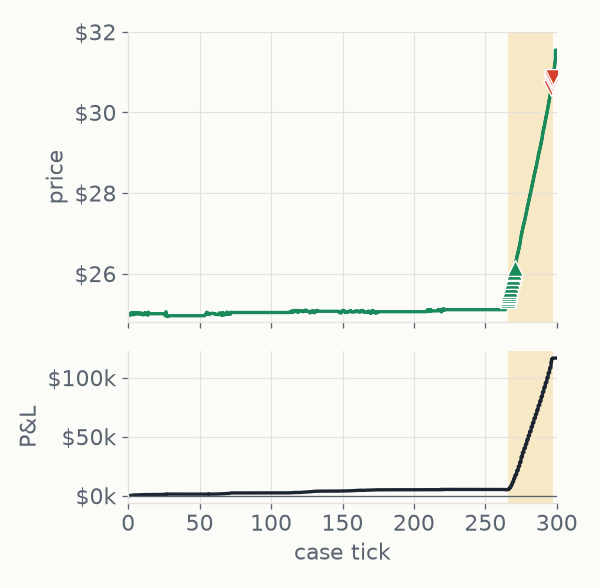
\includegraphics[width=\linewidth]{figures/J_AC.png}\caption{AC: $+\$117$k}\end{subfigure}
\caption{Price (top) and cumulative P\&L (bottom) per stock. Triangles: trend-engine buys and sells; shading: trend mode; dashed line (RY): P\&L without the tick-217 event.}
\label{fig:sec}
\end{figure}

\textbf{What the bot did, stock by stock.}
\begin{itemize}
  \item \textbf{CNR (ticks 3--13): false starts, then the learning rule worked.} The engine took three positions (short, long, short) that reversed almost immediately, losing \$36.7k.
        In the opening seconds CNR's book was thin, with spreads of 11 to 100 ticks and price jumps of 30--100 cents per tick, while the volatility estimate was still at its starting value.
        Noise therefore looked like a trend. Each loss raised CNR's entry bar by $1.4\times$, three losses in a row locked the engine out of CNR, and it never traded CNR directionally again.
        The account-level circuit breaker fired once, at tick 38, flattened everything and paused for eight seconds.
  \item \textbf{RY (ticks 200--218): the system working as designed.} At tick 200 the efficiency ratio jumped from 0 to 1.0, a straight-line move. At tick 201.6 the EMA gap had stayed above 12 ticks
        for 0.8\,s and the trend engine took over. Its first order was about 12{,}000 shares; by tick 210 it held 22{,}062 shares (88\% of the limit), bought between \$100.2 and \$105.5, and the
        wide trailing stop let it ride the drift to \$118. At tick 217 the RY book turned one-sided: the asks vanished and the bids jumped to \$346 and then \$402, following Group~12's activity.
        The engine sold the whole position into those bids in five orders over about four seconds, at an average of roughly \$383.
  \item \textbf{AC (ticks 265--296): a clean trend trade.} AC began a straight climb from \$25.1 to \$31.5. The engine entered at the start, held about 22{,}000 shares and closed in the end-of-case unwind.
\end{itemize}

\textbf{Why market making did not make money, even though prices mean-reverted.} This was the most instructive result. With a one-tick spread, a successful round trip earns about \$0.01 per share
plus the rebate. The inventory stop, however, cuts a losing position once it is down $\max(5\text{ ticks}, 3\sigma)$. With roughly $+1$ tick per winning trade and $-5$ ticks per stopped trade,
the market maker needs about five wins in every six trades just to break even. In this market prices moved in jumps of several cents rather than one-cent wiggles, so stops fired often
(86 times on CNR), and the orders that filled were disproportionately those a moving price ran through (adverse selection). Mean reversion in the \emph{price} is not the same thing as profitable
market making; the spread has to be wide relative to the size of the jumps.

\textbf{Size strategy: be big only when the evidence is strong or the risk is small.}
\begin{itemize}
  \item \textbf{Market-making quotes} were 5{,}000 shares a side in calm markets or healthy 2--6 tick spreads, 3{,}000 normally, half that when stressed, and 2{,}000 in thin books, so quote
        size falls exactly when the risk of being run over rises.
  \item \textbf{The inventory brake} uses $r = |\text{position}|/9{,}000$. The side that would add to the position is multiplied by $e^{-3r}$ and moved away from the market by
        $\operatorname{round}(4r^{1.5})$ ticks, and it is switched off entirely at $r \ge 0.85$ (7{,}650 shares), while the reducing side is enlarged by $(1+r)$. For example, holding
        4{,}500 shares ($r = 0.5$) cuts a 3{,}000-share adding quote to about 700 shares placed one tick further away, and raises the reducing quote to 4{,}500. This is a discrete version of the
        inventory skew in the Avellaneda--Stoikov market-making model.
  \item \textbf{Trend sizing} starts with 60\% of the available capacity and grows with the strength of the signal up to 95\% of the cap (about 22{,}000 shares), in orders of at most 5{,}000.
        The trend engine is the only part allowed to use most of the limit, because it only acts when the evidence is strong, and it carries a trailing stop.
  \item \textbf{Limits and unwinding.} On top of the 93\% pre-trade check, a safety net cuts the largest position immediately if the actual position ever passes 96\% of the limit; the \$40k
        drawdown breaker flattens the book; and about 20\,s before the close the bot stops adding risk and about 8\,s before it crosses to finish flat. After any trend exit the stock sells down in
        an ``exit'' mode with capped limit orders. Over the whole run the peak gross position was 23{,}088 and the peak net position 22{,}837, against a limit of 25{,}000.
\end{itemize}

\textbf{Our Python script and how to use it.} The trading code is listed in the Appendix (\code{algo2e\_strategy.py}). It needs Python 3 and the \code{requests} package. Start the RIT
client with the API enabled, note the API key and port, and run:
\begin{lstlisting}[basicstyle=\ttfamily\footnotesize, frame=single, columns=fullflexible, breaklines=true]
python algo2e_strategy.py <API_KEY> <PORT> [CASE_MINUTES]     # e.g. python algo2e_strategy.py abcde 15000 20
\end{lstlisting}
If started before the case begins, it waits until the case status is \code{ACTIVE}; without \code{CASE\_MINUTES} it learns the length of a tick from the case clock and scales its time windows
accordingly. Every parameter sits in one configuration block at the top of the file. Ctrl-C cancels all orders and flattens the book. While running it prints every fill, mode change and stop,
and once a second a status line per stock with its position, quotes and regime. It writes two logs: \code{logs/v3\_ticks\_*.csv}, one row per loop with prices, signals, positions, modes and P\&L
for every stock, and \code{logs/v3\_events\_*.csv}, every order, cancel, fill and decision with its reason. All numbers in this report come from these logs.
\code{dir.py} (trend engine only) and \code{mm.py} (market making only) are the same code with one engine disabled.

\textbf{Testing before the case.} During development we tested the bot against a fake exchange that reproduces RIT's order latency, position-reporting lag, rebates and fees, with eleven market scenarios. Re-running our development
script through all of them (90\,s each) gave: calm, mean-reverting and slow-grind markets between $-\$932$ and $+\$440$; trending, reversing and crashing markets $+\$41$k to $+\$124$k; spikes, sweeps
and one-sided order flow $+\$12$k to $+\$49$k; and a whipsaw market (short trends that reverse) $-\$44$k. Every run ended flat with peak gross at most 23{,}200 shares. The live result has the same
shape: break-even in calm markets, profits in trends, and the whipsaw case is the same failure mode as CNR's opening.

\textbf{A note on the following round.} In the next round our RIT client crashed, so we had cancelled the script and only started it after the round was under way (it first joined at tick 49 of 300).
It could not run the strategy as designed, and the late session ended with a small loss of \$3{,}427. We mention it for completeness only.

%==========================================================================================
\subsection*{(d) What was your P\&L?}

\textbf{The main strategy finished at \$6,288,771.} This is the server's net liquidation value. It equals the sum of the three stocks' P\&L to the cent, which is what we would expect if no fines were
charged. The two variants ran on separate accounts in the same market and are reported separately:

\vspace{-2pt}
\begin{table}[H]
\centering\footnotesize
\begin{tabular}{lrrrr}
\toprule
 & CNR & RY & AC & Total\\
\midrule
\code{algo2e\_fin.py} (market making + trend; main) & $-\$52{,}646$ & $\$6{,}224{,}827$ & $\$116{,}590$ & \textbf{\$6,288,771}\\
\code{dir.py} (trend engine only) & $-\$77{,}895$ & $\$6{,}238{,}173$ & $\$118{,}130$ & \$6,278,408\\
Market making only & $-\$28{,}719$ & $-\$6{,}147$ & $\$6{,}434$ & $-\$28{,}433$\\
\bottomrule
\end{tabular}
\end{table}
\vspace{-6pt}

\begin{figure}[!htb]
\centering
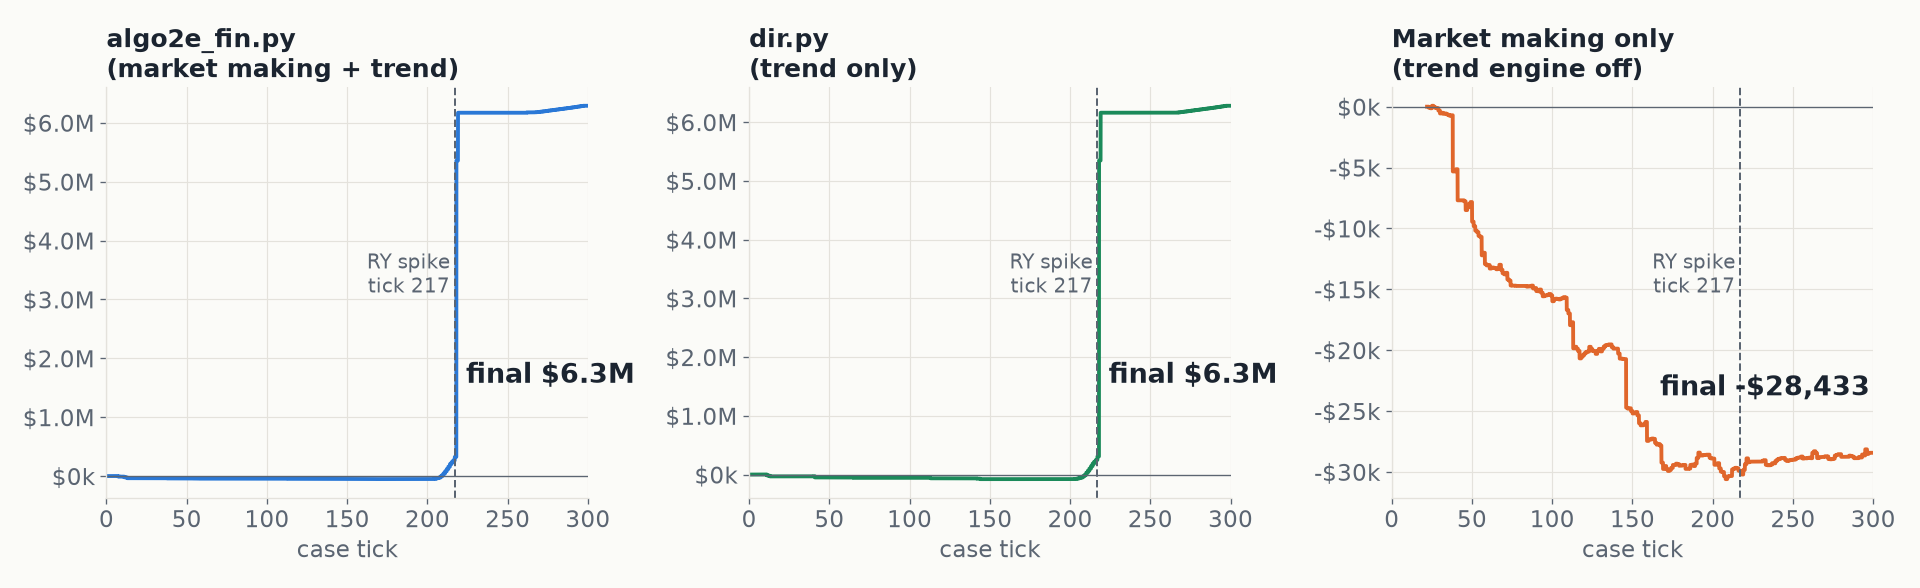
\includegraphics[width=0.8\textwidth]{figures/H3_total_pnl_three_algos.png}
\caption{Total P\&L through the case for the three builds; dashed line: the RY event at tick 217.}
\end{figure}
\vspace{-4pt}

\textbf{Where the money came from.} Splitting the main strategy's P\&L by the mode the bot was in shows a clear division of labour. The trend engine was in control for less than 7\% of the time on any
stock (about 2\% on CNR, 4\% on RY and 6\% on AC) and earned $+\$6.30$M net: $+\$5.78$M from selling RY into the dislocation, $+\$451$k from riding RY's drift before it, $+\$112$k on AC, less \$36k on
CNR's early false starts. Market making, active the rest of the time, finished at about $-\$15$k. Running three builds side by side in the same market makes this a controlled comparison: the same trend
engine produced almost the same result with or without market making, while market making alone lost money. \code{dir.py}'s faster entries (8-tick instead of 12-tick threshold) lost more on CNR,
which illustrates the trade-off between catching a move early and reacting to noise.

\textbf{With and without the RY event.} About 92\% of the profit came from one event, so we also measured what the strategy earned on its own terms. Re-valuing the RY exit at the last normal bid before
the book broke (\$121.08), with everything else unchanged, gives about \textbf{\$511k}, and between \$244k and \$559k for exit prices from \$109 to \$123. This still includes the RY drift that preceded the
event, so it is the optimistic reading; ticks 0--199 on their own were a loss of about \$52k.

\textbf{What the mean-reversion tilt would have added.} Replaying the logged Bollinger z-scores and regime labels, and holding the position the tilt would have targeted, gives about $+\$37$k at 8{,}000
shares and $+\$56$k at 12{,}000 before trading costs, and roughly $+\$5$k to $+\$20$k after them. Almost all of it falls before tick 200, because the tilt switches itself off when a stock is in TREND,
so it would not have been short RY into the event. At under 1\% of the total, this supports our decision to leave it off.

\textbf{How we read the result.} We did not predict the RY event, and we do not claim to have. What the system did was put the right position on by rule before the event: regime detection moved RY
into trend mode within about one case tick of the drift starting, the trend engine sized up to 88\% of the limit, and the volatility-scaled trailing stop kept the position on until the book broke.
The position stayed within limits for the whole case and no fines were charged. The run also showed the two changes we would make first: a warm-up period before the trend engine is allowed to trade,
and fee-aware quoting restricted to stocks where resting orders earn a rebate.
 inside your document.
% Needs in the preamble: amsmath, booktabs, tabularx, graphicx, float, caption, subcaption, xcolor, listings, enumitem
\providecommand{\code}[1]{\texttt{#1}}
\section*{RIT ALGO2e: Strategy Report}
\addcontentsline{toc}{section}{RIT ALGO2e: Strategy Report}
Main strategy: \code{algo2e\_fin.py} (trading code in Appendix~\ref{app:code}).


%==========================================================================================
\subsection*{(a) What was your strategy going in?}

\textbf{The problem.} ALGO2e is a liquidity-provision case: three stocks (CNR $\approx$\$160, RY $\approx$\$100, AC $\approx$\$25), a 25{,}000-share gross and net
limit with fines for breaches, and a fee schedule that pays a rebate for resting orders on two of the three stocks. Market making is the natural way to earn money
here: quote a bid and an ask, collect the spread and the rebate, and keep inventory near zero. It is also the natural way to lose money, because in a trending market
a market maker keeps buying a falling price (or selling a rising one) and ends up holding a large position against the move. We did not know in advance which kind
of market the case would produce. Our working guess was that prices would mostly mean-revert around an anchor, with the possibility of trends or shocks injected during
the case. The strategy therefore had to make money in a calm market, survive a trending one, and switch between the two without anyone touching it.

\textbf{The design: a regime-switching system with three parts.}
\begin{enumerate}
  \item \textbf{Market maker (base income in calm markets).} Passive quotes on every stock, sized according to how volatile the stock currently is, with an
        inventory brake that makes it progressively harder to add to a position and easier to reduce it.
  \item \textbf{Trend engine (insurance against our guess being wrong).} When a stock starts moving steadily in one direction, quoting on that stock stops and
        the engine takes a large position \emph{with} the move, held with a trailing stop that is scaled to the stock's volatility.
  \item \textbf{Risk layer (overrides both).} Only limit orders are used, every order is checked against worst-case exposure before it is sent, and an account-level
        circuit breaker and end-of-case unwind sit on top. Our explicit objective was profit with \emph{zero fines}.
\end{enumerate}
Each stock is handled every pass of the loop (up to 40 times a second) in a fixed order of precedence: end-of-case unwind or circuit breaker first, then the trend engine,
then market-making loss controls, and only then new quotes. The first rule that applies wins, so safety always takes priority over making money.

\textbf{How the bot knows which regime it is in.} For every stock the bot keeps a few simple, robust measurements:
the \emph{EMA gap}, the difference between a fast (1\,s) and a slow (8\,s) exponential moving average of the mid-price, measured in ticks, which says how far the
price has run from its recent past; the \emph{Kaufman efficiency ratio} over 10\,s, $|\text{net move}|/\text{total path}$, which is close to 1 when the price moves in a
straight line and close to 0 when it goes back and forth; the width of its \emph{Bollinger bands} relative to their own 2-minute baseline, which classifies the stock as
calm, normal or stressed; a short-term \emph{volatility} estimate; and a \emph{t-statistic} of the drift over 20 case ticks for slow, grinding trends. A stock is labelled
TREND when the efficiency ratio is at least 0.45 and the move is at least 12 ticks, and it keeps that label until the ratio falls below 0.33. This hysteresis stops the label
from flickering on the boundary. Importantly, the label alone never triggers a trade. The trend engine also requires the EMA gap to exceed $\max(12\text{ ticks}, 5\sigma)$,
the spread to be at most 6 ticks, and the signal to persist for 0.8\,s. Because the thresholds are expressed in units of the stock's own volatility, the same rules work for a
\$25 stock and a \$160 stock, and a noisy stock needs a bigger move before the engine believes it.

\textbf{What we decided against.} We also built a directional mean-reversion tilt: instead of steering inventory to zero, it targets a long position when the price is low in
its Bollinger band and a short one when it is high (up to 8{,}000--12{,}000 shares). In testing it did worse than plain inventory-to-zero market making, because it is holding
inventory against the move at exactly the moment a breakout starts. It was switched off for the graded run (\code{MR\_MAX\_INV = 0}). Several other rules came from our practice
sessions: market orders into a thin AC book lost tens of thousands of dollars in a second, so every aggressive order is a limit order capped within 2\% of fair value; and a
bot that reads its own resting quotes as ``the market'' keeps outbidding itself, so the bot strips its own orders from the book before computing any price.

%==========================================================================================
\subsection*{(b) What changes did you make to handle multiple securities and fees/rebates?}

\textbf{Nothing about the securities is hard-coded.} At start-up the bot reads \code{/securities} for the list of tradeable tickers and each ticker's tick size, taker fee
and maker rebate, and \code{/limits} for the gross and net limits and the fine schedule. Its own caps are derived from these values, so the same script runs unchanged on
two, three or ten securities and on a different limit.

\textbf{Each stock thinks for itself; all stocks share one risk budget.} Every stock has its own signals, regime label, mode (market making, trend, or exiting a trend),
stops, loss pauses and a learned entry threshold that rises after losing trend trades on that stock. What the stocks cannot each have is their own limit, because the
25{,}000-share limit is shared. We handled this in four ways:
\begin{itemize}
  \item \textbf{Aggregate worst-case check.} Before any order is sent, the bot assumes that every resting order, every order still in flight and the new order all fill at once,
        summed across all stocks, and requires gross and net exposure to stay below 93\% of the limit (23{,}250 shares). If the order does not fit, it is shrunk by 40\% at a time
        and dropped if it still does not fit.
  \item \textbf{Capacity allocation.} The trend engine's maximum size on one stock is $0.95\times$ the cap minus whatever is held in the other stocks. When RY's trend started the
        other books were almost flat, so RY could take about 22{,}000 shares; had AC been trending at the same time, RY would have received only what was left.
  \item \textbf{Per-stock inventory caps.} Market-making inventory is limited to 9{,}000 shares per stock, so one stock cannot absorb the whole budget through passive fills.
  \item \textbf{Priority when room is tight.} Aggressive orders (stops, trend trades, unwind) are processed first, then the quotes of the stock with the healthiest wide spread,
        which is the most profitable to quote, then the remaining quotes.
\end{itemize}
Order books for all stocks are fetched in parallel so that adding a stock does not slow the loop. Because RIT confirms orders and updates positions with a delay, the bot keeps its own
registry of orders: a just-sent order counts as live before RIT lists it, and an order that has disappeared still counts toward exposure for a second, until the position catches up.

\textbf{Fees and rebates.} The useful way to read the fee schedule is as a fraction of the one-tick (\$0.01) spread, because that is all a market maker earns per share:

\vspace{-2pt}
\begin{table}[H]
\centering\footnotesize
\begin{tabular}{lrrl}
\toprule
 & Maker rebate (resting) & Taker fee (crossing) & What it means for us\\
\midrule
CNR & $+\$0.0023$ (23\% of a tick) & \$0.0027 (27\% of a tick) & rest; crossing costs $>$\,\textonequarter\ of the spread\\
AC  & $+\$0.0011$ (11\%) & \$0.0015 (15\%) & rest\\
RY  & $-\$0.0020$ (resting \emph{pays} 20\%) & $-\$0.0014$ (crossing \emph{earns} 14\%) & resting costs; crossing is cheap\\
\bottomrule
\end{tabular}
\end{table}
\vspace{-4pt}
A 1{,}000-share round trip on CNR earns \$10 of spread plus \$4.60 of rebates if both sides rest, but crossing both sides would cost the \$10 spread plus \$5.40 in fees. That asymmetry
drove three choices. First, \textbf{passive-first execution}: market making only rests orders, and we cross the spread only when we must (stops, trend entries and exits, the final unwind),
always with capped limit orders. Second, \textbf{size where the economics are best}: full size (5{,}000 shares a side) is quoted only when the market is calm or the spread is a
``healthy'' 2--6 ticks, where spread plus rebate can pay for the inventory risk; on a 2-tick spread we step inside only on the side that reduces our position. Third,
\textbf{RY is different}: resting there costs money, so market making on RY is structurally weak, while our RY trend trades were executed aggressively, which is the cheaper side on that stock.
In this version the fee schedule shaped the design rather than entering the quoting formula itself; making quotes explicitly fee-aware, for example not resting on RY at all, is the
first change we would make.

%==========================================================================================
\subsection*{(c) What happened during the simulation? What was your size strategy?}

\textbf{The market we got.} For the first 200 case ticks all three prices behaved like mean-reverting series. Their 10-tick variance ratios were 0.19--0.26 (a random walk scores 1),
and consecutive returns were negatively correlated ($-0.21$ to $-0.33$), so our working assumption held for two-thirds of the case. After tick 200 the picture changed: RY broke out,
AC trended steadily, and CNR stayed inside its band to the end (Figure~\ref{fig:sec}).

\begin{figure}[!htb]
\centering\hspace*{0.05\textwidth}
\begin{subfigure}{0.27\textwidth}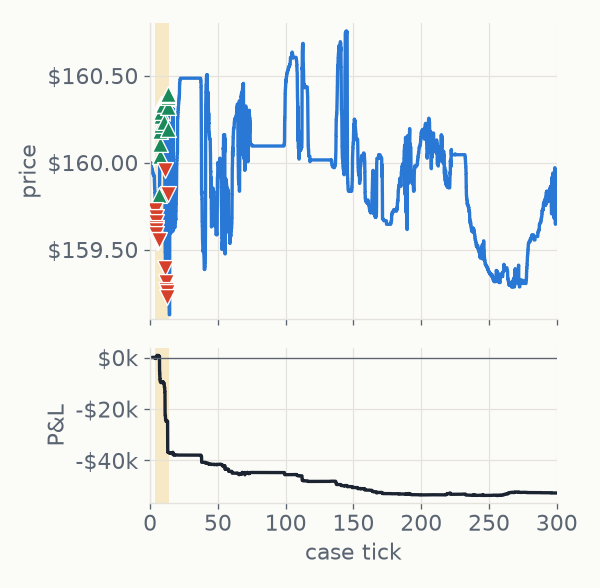
\includegraphics[width=\linewidth]{figures/J_CNR.png}\caption{CNR: $-\$53$k}\end{subfigure}\hfill
\begin{subfigure}{0.27\textwidth}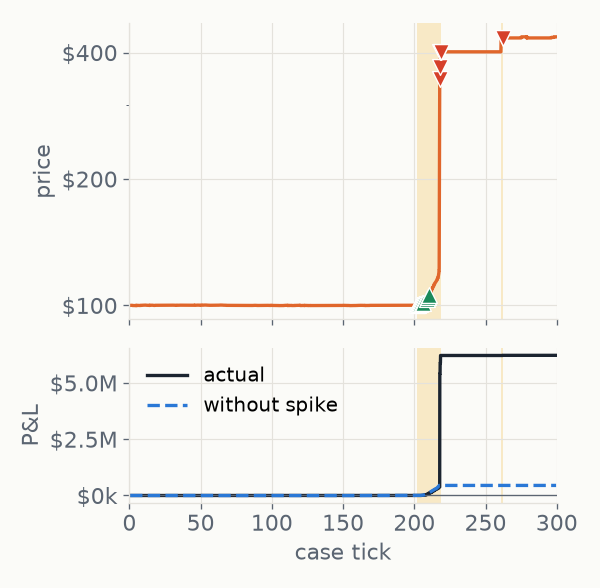
\includegraphics[width=\linewidth]{figures/J_RY.png}\caption{RY: $+\$6.22$M}\end{subfigure}\hfill
\begin{subfigure}{0.27\textwidth}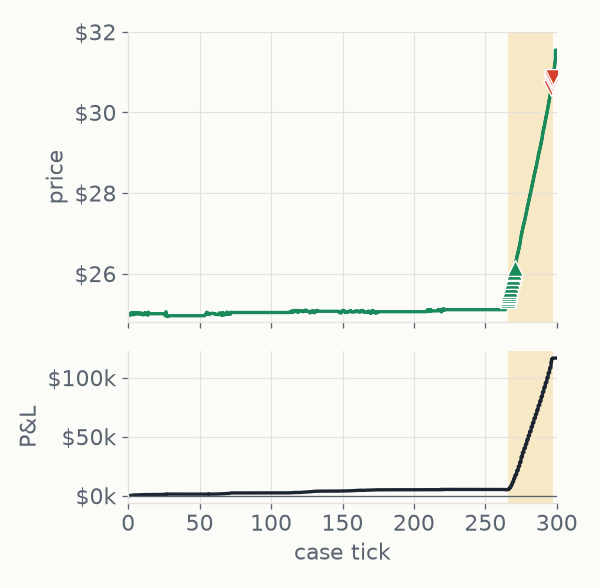
\includegraphics[width=\linewidth]{figures/J_AC.png}\caption{AC: $+\$117$k}\end{subfigure}
\caption{Price (top) and cumulative P\&L (bottom) per stock. Triangles: trend-engine buys and sells; shading: trend mode; dashed line (RY): P\&L without the tick-217 event.}
\label{fig:sec}
\end{figure}

\textbf{What the bot did, stock by stock.}
\begin{itemize}
  \item \textbf{CNR (ticks 3--13): false starts, then the learning rule worked.} The engine took three positions (short, long, short) that reversed almost immediately, losing \$36.7k.
        In the opening seconds CNR's book was thin, with spreads of 11 to 100 ticks and price jumps of 30--100 cents per tick, while the volatility estimate was still at its starting value.
        Noise therefore looked like a trend. Each loss raised CNR's entry bar by $1.4\times$, three losses in a row locked the engine out of CNR, and it never traded CNR directionally again.
        The account-level circuit breaker fired once, at tick 38, flattened everything and paused for eight seconds.
  \item \textbf{RY (ticks 200--218): the system working as designed.} At tick 200 the efficiency ratio jumped from 0 to 1.0, a straight-line move. At tick 201.6 the EMA gap had stayed above 12 ticks
        for 0.8\,s and the trend engine took over. Its first order was about 12{,}000 shares; by tick 210 it held 22{,}062 shares (88\% of the limit), bought between \$100.2 and \$105.5, and the
        wide trailing stop let it ride the drift to \$118. At tick 217 the RY book turned one-sided: the asks vanished and the bids jumped to \$346 and then \$402, following Group~12's activity.
        The engine sold the whole position into those bids in five orders over about four seconds, at an average of roughly \$383.
  \item \textbf{AC (ticks 265--296): a clean trend trade.} AC began a straight climb from \$25.1 to \$31.5. The engine entered at the start, held about 22{,}000 shares and closed in the end-of-case unwind.
\end{itemize}

\textbf{Why market making did not make money, even though prices mean-reverted.} This was the most instructive result. With a one-tick spread, a successful round trip earns about \$0.01 per share
plus the rebate. The inventory stop, however, cuts a losing position once it is down $\max(5\text{ ticks}, 3\sigma)$. With roughly $+1$ tick per winning trade and $-5$ ticks per stopped trade,
the market maker needs about five wins in every six trades just to break even. In this market prices moved in jumps of several cents rather than one-cent wiggles, so stops fired often
(86 times on CNR), and the orders that filled were disproportionately those a moving price ran through (adverse selection). Mean reversion in the \emph{price} is not the same thing as profitable
market making; the spread has to be wide relative to the size of the jumps.

\textbf{Size strategy: be big only when the evidence is strong or the risk is small.}
\begin{itemize}
  \item \textbf{Market-making quotes} were 5{,}000 shares a side in calm markets or healthy 2--6 tick spreads, 3{,}000 normally, half that when stressed, and 2{,}000 in thin books, so quote
        size falls exactly when the risk of being run over rises.
  \item \textbf{The inventory brake} uses $r = |\text{position}|/9{,}000$. The side that would add to the position is multiplied by $e^{-3r}$ and moved away from the market by
        $\operatorname{round}(4r^{1.5})$ ticks, and it is switched off entirely at $r \ge 0.85$ (7{,}650 shares), while the reducing side is enlarged by $(1+r)$. For example, holding
        4{,}500 shares ($r = 0.5$) cuts a 3{,}000-share adding quote to about 700 shares placed one tick further away, and raises the reducing quote to 4{,}500. This is a discrete version of the
        inventory skew in the Avellaneda--Stoikov market-making model.
  \item \textbf{Trend sizing} starts with 60\% of the available capacity and grows with the strength of the signal up to 95\% of the cap (about 22{,}000 shares), in orders of at most 5{,}000.
        The trend engine is the only part allowed to use most of the limit, because it only acts when the evidence is strong, and it carries a trailing stop.
  \item \textbf{Limits and unwinding.} On top of the 93\% pre-trade check, a safety net cuts the largest position immediately if the actual position ever passes 96\% of the limit; the \$40k
        drawdown breaker flattens the book; and about 20\,s before the close the bot stops adding risk and about 8\,s before it crosses to finish flat. After any trend exit the stock sells down in
        an ``exit'' mode with capped limit orders. Over the whole run the peak gross position was 23{,}088 and the peak net position 22{,}837, against a limit of 25{,}000.
\end{itemize}

\textbf{Our Python script and how to use it.} The trading code is listed in the Appendix (\code{algo2e\_strategy.py}). It needs Python 3 and the \code{requests} package. Start the RIT
client with the API enabled, note the API key and port, and run:
\begin{lstlisting}[basicstyle=\ttfamily\footnotesize, frame=single, columns=fullflexible, breaklines=true]
python algo2e_strategy.py <API_KEY> <PORT> [CASE_MINUTES]     # e.g. python algo2e_strategy.py abcde 15000 20
\end{lstlisting}
If started before the case begins, it waits until the case status is \code{ACTIVE}; without \code{CASE\_MINUTES} it learns the length of a tick from the case clock and scales its time windows
accordingly. Every parameter sits in one configuration block at the top of the file. Ctrl-C cancels all orders and flattens the book. While running it prints every fill, mode change and stop,
and once a second a status line per stock with its position, quotes and regime. It writes two logs: \code{logs/v3\_ticks\_*.csv}, one row per loop with prices, signals, positions, modes and P\&L
for every stock, and \code{logs/v3\_events\_*.csv}, every order, cancel, fill and decision with its reason. All numbers in this report come from these logs.
\code{dir.py} (trend engine only) and \code{mm.py} (market making only) are the same code with one engine disabled.

\textbf{Testing before the case.} During development we tested the bot against a fake exchange that reproduces RIT's order latency, position-reporting lag, rebates and fees, with eleven market scenarios. Re-running our development
script through all of them (90\,s each) gave: calm, mean-reverting and slow-grind markets between $-\$932$ and $+\$440$; trending, reversing and crashing markets $+\$41$k to $+\$124$k; spikes, sweeps
and one-sided order flow $+\$12$k to $+\$49$k; and a whipsaw market (short trends that reverse) $-\$44$k. Every run ended flat with peak gross at most 23{,}200 shares. The live result has the same
shape: break-even in calm markets, profits in trends, and the whipsaw case is the same failure mode as CNR's opening.

\textbf{A note on the following round.} In the next round our RIT client crashed, so we had cancelled the script and only started it after the round was under way (it first joined at tick 49 of 300).
It could not run the strategy as designed, and the late session ended with a small loss of \$3{,}427. We mention it for completeness only.

%==========================================================================================
\subsection*{(d) What was your P\&L?}

\textbf{The main strategy finished at \$6,288,771.} This is the server's net liquidation value. It equals the sum of the three stocks' P\&L to the cent, which is what we would expect if no fines were
charged. The two variants ran on separate accounts in the same market and are reported separately:

\vspace{-2pt}
\begin{table}[H]
\centering\footnotesize
\begin{tabular}{lrrrr}
\toprule
 & CNR & RY & AC & Total\\
\midrule
\code{algo2e\_fin.py} (market making + trend; main) & $-\$52{,}646$ & $\$6{,}224{,}827$ & $\$116{,}590$ & \textbf{\$6,288,771}\\
\code{dir.py} (trend engine only) & $-\$77{,}895$ & $\$6{,}238{,}173$ & $\$118{,}130$ & \$6,278,408\\
Market making only & $-\$28{,}719$ & $-\$6{,}147$ & $\$6{,}434$ & $-\$28{,}433$\\
\bottomrule
\end{tabular}
\end{table}
\vspace{-6pt}

\begin{figure}[!htb]
\centering
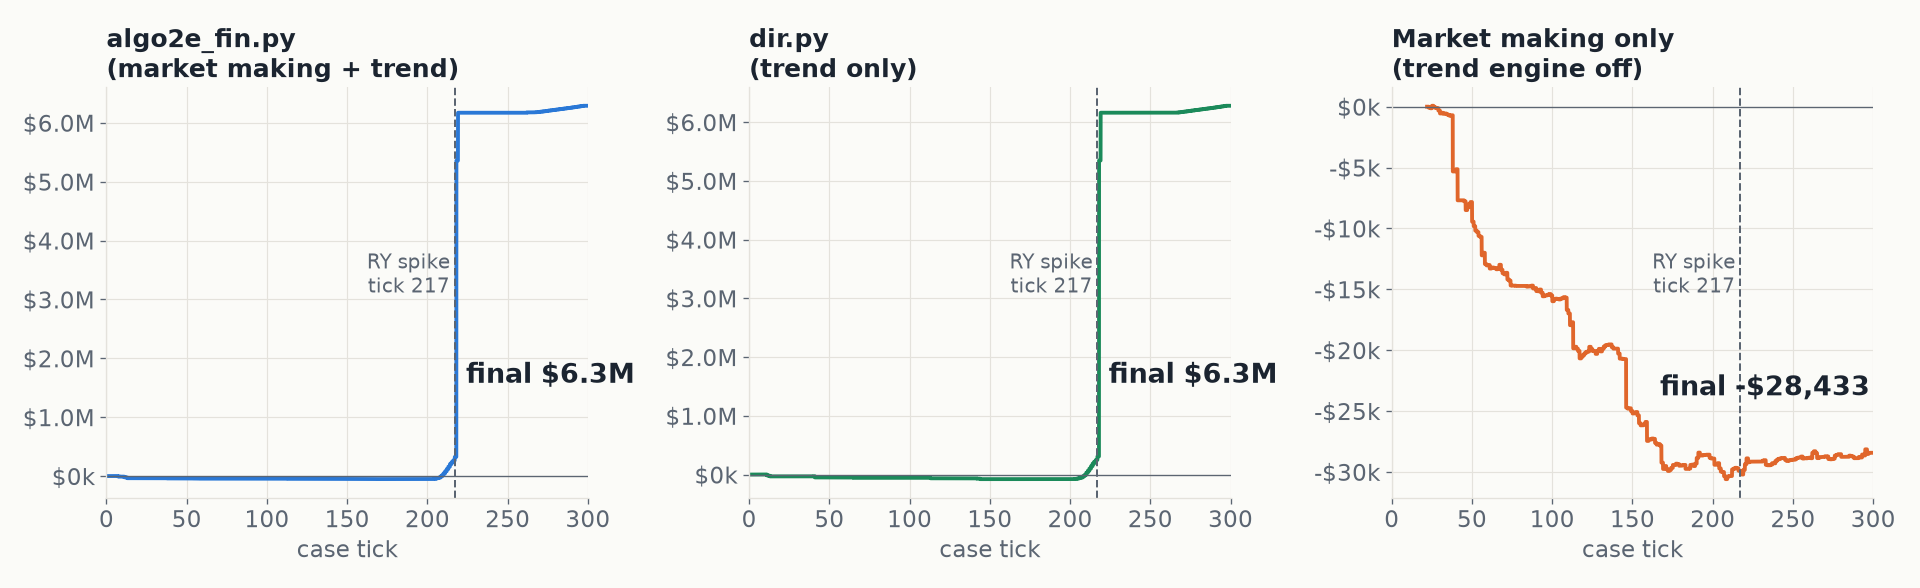
\includegraphics[width=0.8\textwidth]{figures/H3_total_pnl_three_algos.png}
\caption{Total P\&L through the case for the three builds; dashed line: the RY event at tick 217.}
\end{figure}
\vspace{-4pt}

\textbf{Where the money came from.} Splitting the main strategy's P\&L by the mode the bot was in shows a clear division of labour. The trend engine was in control for less than 7\% of the time on any
stock (about 2\% on CNR, 4\% on RY and 6\% on AC) and earned $+\$6.30$M net: $+\$5.78$M from selling RY into the dislocation, $+\$451$k from riding RY's drift before it, $+\$112$k on AC, less \$36k on
CNR's early false starts. Market making, active the rest of the time, finished at about $-\$15$k. Running three builds side by side in the same market makes this a controlled comparison: the same trend
engine produced almost the same result with or without market making, while market making alone lost money. \code{dir.py}'s faster entries (8-tick instead of 12-tick threshold) lost more on CNR,
which illustrates the trade-off between catching a move early and reacting to noise.

\textbf{With and without the RY event.} About 92\% of the profit came from one event, so we also measured what the strategy earned on its own terms. Re-valuing the RY exit at the last normal bid before
the book broke (\$121.08), with everything else unchanged, gives about \textbf{\$511k}, and between \$244k and \$559k for exit prices from \$109 to \$123. This still includes the RY drift that preceded the
event, so it is the optimistic reading; ticks 0--199 on their own were a loss of about \$52k.

\textbf{What the mean-reversion tilt would have added.} Replaying the logged Bollinger z-scores and regime labels, and holding the position the tilt would have targeted, gives about $+\$37$k at 8{,}000
shares and $+\$56$k at 12{,}000 before trading costs, and roughly $+\$5$k to $+\$20$k after them. Almost all of it falls before tick 200, because the tilt switches itself off when a stock is in TREND,
so it would not have been short RY into the event. At under 1\% of the total, this supports our decision to leave it off.

\textbf{How we read the result.} We did not predict the RY event, and we do not claim to have. What the system did was put the right position on by rule before the event: regime detection moved RY
into trend mode within about one case tick of the drift starting, the trend engine sized up to 88\% of the limit, and the volatility-scaled trailing stop kept the position on until the book broke.
The position stayed within limits for the whole case and no fines were charged. The run also showed the two changes we would make first: a warm-up period before the trend engine is allowed to trade,
and fee-aware quoting restricted to stocks where resting orders earn a rebate.
